% 05_results_b.tex  (Writer D)  Results, part 2: Sections 4.6-4.8. Continues \section{Results} of 04_results_a.tex.
% Every number is copied from docs/RESULTS_LOG.md (L = line), the fact sheet (facts), the stored report of the
% final run (report60 = scratchpad/report60.md, line numbers) or paper/v5/paper.tex (v5 P = line).
% Template (round 2): shares in per cent; differences between shares in percentage points (stored proportion
% difference and its bounds times 100, nothing else); ESG, natural ESG and Youden index on the 0 to 1 scale;
% positive differences unsigned.

\subsection{Unedited image pairs: the advantage did not carry over, and detection improved only with unedited training images}
\label{subsec:res_pairs}

On 103 unedited pairs from REAL-Colon, a polyp frame and a polyp-free frame of the same video received the same question (Section~\ref{subsec:pairs}). The natural ESG of \ms{} was $0.243$ $\ci{0.149}{0.340}$, the same as that of its base model (difference $0.000$ $\ci{-0.103}{0.095}$) and lower than that of \gem{} ($0.466$; $-0.223$ $\ci{-0.346}{-0.102}$) and \opus{} ($0.447$; $-0.204$ $\ci{-0.333}{-0.071}$); the pre-specified criterion was not met (Table~\ref{tab:natural}; Supplementary Table~\ref{tab:s_realcolon}). \ms{} reported a polyp on 2 of 103 polyp-free frames, against 15 for its base model, but it requested a better image on 12 more, and the share answered ``absent'' or referred was the same (86.4\% against 85.4\%). It reported the polyp on 36 of 103 polyp frames, against 40.
% src: L1458-1468 (natural ESG, differences, criterion); L1484-1489 (2/103, 15/103, 12 requests, 89/103 = 86.4%, 36/103, 40/103)

A two-by-two comparison of first-stage models, trained with or without counterfactual views and with or without unedited pairs, separated the two kinds of training image (one seed; Supplementary Table~\ref{tab:s_twobytwo}). Natural ESG was $0.563$ with unedited pairs only, $0.505$ with both kinds, $0.223$ with counterfactual views only and $0.214$ with neither. Unedited pairs raised it by $0.350$ $\ci{0.227}{0.474}$ without counterfactual views and by $0.282$ $\ci{0.156}{0.405}$ with them. Counterfactual views were not shown to add to it once unedited pairs were in training ($-0.058$ $\ci{-0.168}{0.042}$, $p = 0.311$; the pre-specified comparison). Without unedited pairs, they raised the share of polyp-free frames answered ``absent'' or referred (86.4\% against 68.9\%; a polyp reported on 3 against 27 of 103) and lowered the share of polyp frames found (35.9\% against 52.4\%). On the main test, ESG was $0.744$ with both kinds and $0.260$ with unedited pairs only (difference $0.484$ $\ci{0.408}{0.558}$).
% src: L1997-2026; facts C7 (two-by-two table: found 35.9% and 52.4%, absent or referred 86.4% and 68.9%, polyp reported 3 and 27) and C1 (main test)

\begin{table*}[!t]
\caption{Unedited colonoscopy pairs: a polyp frame and a polyp-free frame of the same video or clip, both asked ``Is there a polyp in this image?''. REAL-Colon: 103 pairs from 46 videos of four centres; the answers of \msn{} are cross-validated (each pair is answered by a copy trained without that pair's video). LDPolypVideo: 116 pairs from 160 clips of one hospital, none of whose images was used to train or select any of our models. Found: the polyp frame was not answered ``absent'' and was not referred; a request for a better image therefore counts as found. Absent or referred: the answer to the polyp-free frame. Natural ESG: the share of polyp-free frames answered ``absent'' or referred minus the same share for polyp frames. Brackets give 95\% intervals from $2{,}000$ bootstrap resamples of whole videos or clips. Differences are \msn{} minus the row model, paired over the same pairs, with two-sided $p$ values. \msn{} is the model of the first training seed; the majority vote of its three seeds scored $0.586$ $\ci{0.491}{0.673}$ on LDPolypVideo. The differences of \ms{} from the other models on REAL-Colon are in Supplementary Table~\ref{tab:s_realcolon}. --: not applicable.}
\label{tab:natural}
\centering
\footnotesize
\setlength{\tabcolsep}{3.5pt}
\begin{adjustbox}{max width=\textwidth}
\begin{tabular}{l cccc cccc}
\toprule
 & \multicolumn{4}{c}{REAL-Colon ($103$ pairs)} & \multicolumn{4}{c}{LDPolypVideo ($116$ pairs)} \\
\cmidrule(lr){2-5}\cmidrule(lr){6-9}
Model & \shortstack{Polyp\\frames\\found} & \shortstack{Polyp-free\\frames absent\\or referred} & \shortstack{Natural ESG\\{}[95\% CI]} & \shortstack{\msn{} minus model\\{}[95\% CI], $p$} & \shortstack{Polyp\\frames\\found} & \shortstack{Polyp-free\\frames absent\\or referred} & \shortstack{Natural ESG\\{}[95\% CI]} & \shortstack{\msn{} minus model\\{}[95\% CI], $p$} \\
\midrule
\base{} & $38.8\%$ & $85.4\%$ & $0.243$ $\ci{0.143}{0.350}$ & $0.291$ $\ci{0.167}{0.407}$, $<0.001$ & $40.5\%$ & $95.7\%$ & $0.362$ $\ci{0.276}{0.448}$ & $0.250$ $\ci{0.155}{0.353}$, $<0.001$ \\
\ms{} & $37.9\%$ & $86.4\%$ & $0.243$ $\ci{0.149}{0.340}$ & $0.291$ $\ci{0.176}{0.402}$, $<0.001$ & $45.7\%$ & $96.6\%$ & $0.422$ $\ci{0.328}{0.517}$ & $0.190$ $\ci{0.112}{0.267}$, $<0.001$ \\
\msn{} & $64.1\%$ & $89.3\%$ & $0.534$ $\ci{0.394}{0.661}$ & -- & $62.1\%$ & $99.1\%$ & $0.612$ $\ci{0.526}{0.698}$ & -- \\
\midrule
\gem{} & $68.0\%$ & $78.6\%$ & $0.466$ $\ci{0.336}{0.581}$ & $0.068$ $\ci{-0.069}{0.202}$, $0.347$ & $71.6\%$ & $81.0\%$ & $0.526$ $\ci{0.422}{0.621}$ & $0.086$ $\ci{-0.017}{0.190}$, $0.117$ \\
\opus{} & $70.9\%$ & $73.8\%$ & $0.447$ $\ci{0.317}{0.579}$ & $0.087$ $\ci{-0.049}{0.230}$, $0.259$ & $62.9\%$ & $83.6\%$ & $0.466$ $\ci{0.362}{0.569}$ & $0.147$ $\ci{0.043}{0.250}$, $0.010$ \\
\gpt{} & $64.1\%$ & $68.0\%$ & $0.320$ $\ci{0.212}{0.437}$ & $0.214$ $\ci{0.071}{0.343}$, $0.003$ & $55.2\%$ & $75.0\%$ & $0.302$ $\ci{0.198}{0.405}$ & $0.310$ $\ci{0.181}{0.431}$, $<0.001$ \\
\bottomrule
\end{tabular}
\end{adjustbox}
\end{table*}
% src: REAL-Colon columns report60 L117-126 (= L1458-1465, L2162-2165); LDPolypVideo columns report60 L69-80 (= L2145-2156); vote report60 L74; a p value of 0.000 in the report is printed as < 0.001

\msn{} is a post hoc model: \msp{} with unedited colonoscopy frames and chest films added to its training (Section~\ref{subsec:models}). On 116 pairs from LDPolypVideo, a hospital not used to train or select our models, it answered ``absent'' or referred on 99.1\% of the polyp-free frames, against 75.0\% to 83.6\% for the reference models, while finding 62.1\% of the polyp frames (reference models 55.2\% to 71.6\%; Fig.~\ref{fig:natural}). Its natural ESG was $0.612$ $\ci{0.526}{0.698}$, higher than that of \ms{} ($0.422$; difference $0.190$ $\ci{0.112}{0.267}$, $p < 0.001$), \opus{} ($0.466$; $0.147$ $\ci{0.043}{0.250}$, $p = 0.010$) and \gpt{} ($0.302$; $0.310$ $\ci{0.181}{0.431}$, $p < 0.001$). A difference from \gem{} ($0.526$) was not shown ($0.086$ $\ci{-0.017}{0.190}$, $p = 0.117$), so by the pre-specified rule the result is mixed. The other two training seeds scored $0.578$ and $0.578$ (Supplementary Table~\ref{tab:s_ldpolyp}).
% src: L2145-2159; facts C9; report60 L69-80 (seeds 1 and 2: 0.578, 0.578); verdict "MIXED" L2145

\begin{figure*}[!t]
\centering
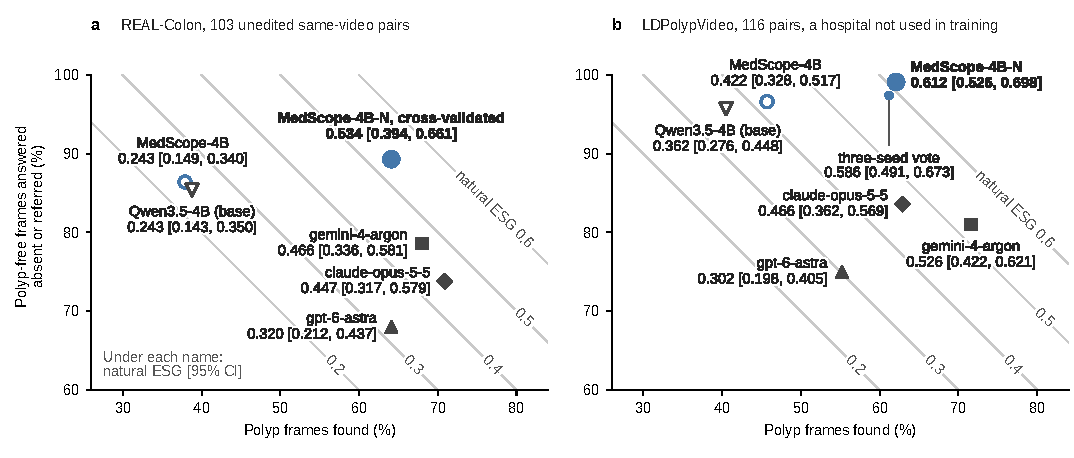
\includegraphics[width=\textwidth]{figures/fig4_natural_pairs.pdf}
\caption{Unedited colonoscopy pairs, by model. (a) REAL-Colon, 103 pairs from 46 videos; the answers of \msn{} are cross-validated. (b) LDPolypVideo, 116 pairs from 160 clips of a hospital not used to train or select any of our models. Each point places a model by the share of polyp frames it found (not answered ``absent'' and not referred, so a request for a better image counts as found) and the share of polyp-free frames it answered ``absent'' or referred. Natural ESG is the sum of the two shares minus one; grey diagonals join points of equal natural ESG, and the value under each name is the natural ESG with its 95\% interval ($2{,}000$ bootstrap resamples of whole videos or clips). The small filled circle in (b) is the three-seed majority vote of \msn{}. Values are in Table~\ref{tab:natural}.}
\label{fig:natural}
\end{figure*}
% src: same numbers as Table tab:natural

On the REAL-Colon pairs, which had already been used to test \ms{}, cross-validated \msn{} scored $0.534$ $\ci{0.394}{0.661}$. This was higher than \ms{} (difference $0.291$ $\ci{0.176}{0.402}$, $p < 0.001$) and \gpt{} ($0.214$ $\ci{0.071}{0.343}$, $p = 0.003$) and not shown to differ from \gem{} ($0.068$ $\ci{-0.069}{0.202}$, $p = 0.347$) or \opus{} ($0.087$ $\ci{-0.049}{0.230}$, $p = 0.259$). An earlier model with only the colonoscopy frames added scored $0.495$ $\ci{0.370}{0.612}$ when every video of the tested centre was withheld from training; context-matched frames and chest X-ray follow-up pairs are in Supplementary Tables~\ref{tab:s_loco} to~\ref{tab:s_cxrpairs}.
% src: L2162-2165; report60 L119-126; L1867-1869 (centre withheld: 0.495 [0.370, 0.612])

\subsection{\texorpdfstring{\msn}{MedScope-4B-N} on the earlier tests and on chest films}
\label{subsec:res_nmodel}

On the main test \msn{} was not shown to differ from \ms{}: ESG was $0.744$ against $0.758$ (difference $-0.014$ $\ci{-0.068}{0.040}$). The pre-specified criterion for a loss, an ESG lower by more than $0.05$, was not met, although the interval does not exclude a fall of that size (Table~\ref{tab:nmodel}). Each of its three training seeds exceeded each reference model in ESG ($0.744$, $0.740$ and $0.726$; smallest difference $0.256$ $\ci{0.171}{0.338}$; Supplementary Table~\ref{tab:s_nseeds}). On the external datasets its ESG was higher than that of \ms{} ($0.672$ against $0.597$; difference $0.076$ $\ci{0.009}{0.143}$, $p = 0.033$) and lower than that of \msp{} ($0.739$; $-0.067$ $\ci{-0.126}{-0.009}$, $p = 0.025$).
% src: L2141-2143; report60 L24, L226 (main test); L2127-2139, report60 L461 (seeds; smallest difference: third seed minus gemini-4-argon); L2185-2186, report60 L291, L296 (external datasets)

On the fresh external set \msn{} was correct on more lesion images than \ms{} (60.7\% against 47.6\%; difference 13.1 percentage points $\ci{6.9}{19.7}$) and reported 22.0\% of erased lesions, against 11.3\% for \msp{} (difference 10.7 percentage points $\ci{5.4}{16.2}$) and 8.3\% for \ms{} (13.7 $\ci{7.7}{20.2}$). The increase was largest on chest films (33\% against 10\%; by source in Supplementary Table~\ref{tab:s_source}), and the training mix that validation did not select reported 17.3\%. Beside \gem{} on this set, \msn{} reported fewer erased lesions (22.0\% against 31.5\%), had a lower ESG ($0.381$ against $0.435$) and was correct on fewer lesion images (60.7\% against 74.1\%); these three contrasts were not tested.
% src: L2178-2183, L2189-2191; report60 L267-268, L273 (0.131 [0.069, 0.197]; 0.137 [0.077, 0.202]; 0.107 [0.054, 0.162], each times 100), L340-347 (chest films 0.33 against 0.10); gemini-4-argon on the fresh external set: L1683 and v5 P1367 (lesion images correct 0.741, ESG 0.435, erased-lesion claims 31.5%)

On unedited chest films \msn{} exceeded all three reference models. On 300 pneumothorax films and 300 films without pneumothorax from CheXthought, from patients not used in training and from the source of part of its training films, its Youden index was $0.660$ $\ci{0.591}{0.726}$. The reference models scored $0.460$, $0.207$ and $0.377$ (differences $0.200$ $\ci{0.122}{0.284}$, $0.453$ $\ci{0.344}{0.560}$ and $0.283$ $\ci{0.196}{0.375}$ for \gem{}, \opus{} and \gpt{}; each $p < 0.001$). Pneumothorax detection on new SIIM-ACR patients, a test used before with the earlier models, was not raised over \msp{} by the first seed (54 against 53 of 100; difference 1.0 percentage point $\ci{-8.0}{10.0}$). The other seeds found 75 and 70, with more reports on erased films (25.0\%, 59.0\% and 43.0\% for the three seeds).
% src: L2174-2176, facts C6, report60 L206-216 (CheXthought); L2169-2172, report60 L22, L196 (0.010 [-0.080, 0.100] times 100), L405-411 (erased-lesion claims by seed on new SIIM-ACR patients: 0.250, 0.590, 0.430)

\begin{table*}[!t]
\caption{\ms{}, the post hoc model \msn{} and \gem{} on each test set. Point estimates; intervals, paired differences, \msp{} and the three-seed vote are in Supplementary Tables~\ref{tab:s_nmodel}, \ref{tab:s_nseeds} and~\ref{tab:s_chest}. ESG: evidence sensitivity gap. Lesion images correct: share of original and control-edited lesion images answered correctly; for the two sets of chest films this column gives the share of unedited pneumothorax films reported as showing a pneumothorax. Youden index: that share plus the share of films without pneumothorax answered ``absent'' or referred, minus one. The CheXthought films have no erased version. --: not applicable, or model not run on the set.}
\label{tab:nmodel}
\centering
\footnotesize
\setlength{\tabcolsep}{4pt}
\begin{adjustbox}{max width=\textwidth}
\begin{tabular}{l ccc ccc ccc ccc}
\toprule
 & \multicolumn{3}{c}{ESG} & \multicolumn{3}{c}{Erased-lesion claims} & \multicolumn{3}{c}{Lesion images correct} & \multicolumn{3}{c}{Youden index} \\
\cmidrule(lr){2-4}\cmidrule(lr){5-7}\cmidrule(lr){8-10}\cmidrule(lr){11-13}
Test set & \ms{} & \msn{} & \gem{} & \ms{} & \msn{} & \gem{} & \ms{} & \msn{} & \gem{} & \ms{} & \msn{} & \gem{} \\
\midrule
Main test ($507$ cases) & $0.758$ & $0.744$ & $0.470$ & $9.6\%$ & $9.1\%$ & $41.1\%$ & $84.9\%$ & $84.7\%$ & $87.4\%$ & -- & -- & -- \\
External datasets ($169$ cases) & $0.597$ & $0.672$ & $0.370$ & $11.8\%$ & $10.9\%$ & $58.8\%$ & $72.7\%$ & $77.7\%$ & $95.0\%$ & -- & -- & -- \\
Fresh internal set ($76$ cases) & $0.472$ & $0.417$ & $0.056$ & $19.4\%$ & $25.0\%$ & $61.1\%$ & $68.1\%$ & $68.1\%$ & $63.9\%$ & -- & -- & -- \\
Fresh external set ($316$ cases) & $0.393$ & $0.381$ & $0.435$ & $8.3\%$ & $22.0\%$ & $31.5\%$ & $47.6\%$ & $60.7\%$ & $74.1\%$ & -- & -- & -- \\
New SIIM-ACR patients ($100 + 100$ films) & $0.000$ & $0.270$ & -- & $0.0\%$ & $25.0\%$ & -- & $0$ of $100$ & $54$ of $100$ & -- & $0.000$ & $0.500$ & -- \\
CheXthought test patients ($300 + 300$ films) & -- & -- & -- & -- & -- & -- & $0.0\%$ & $75.0\%$ & $62.0\%$ & $0.000$ & $0.660$ & $0.460$ \\
\bottomrule
\end{tabular}
\end{adjustbox}
\end{table*}
% src: MedScope-4B and MedScope-4B-N: Supplementary Table tab:s_nmodel (report60 L225-228, L265-268, L290-293, L310-313; lesion images correct and claims are the report's proportions times 100); new SIIM-ACR patients: report60 L190, L197, L407-411 and L1600-1602 (MedScope-4B: ESG 0.000, erased-lesion claims 0.000); CheXthought: report60 L206, L212, L214. gemini-4-argon: main test L486-493 (facts C: 0.874, 0.470, 41.1%); external datasets, fresh internal and fresh external v5 P1359, P1363, P1367 (0.950, 0.370, 58.8; 0.639, 0.056, 61.1; 0.741, 0.435, 31.5; = L1683 for the fresh external set)

\subsection{Alternative training designs and decision rules}
\label{subsec:res_designs}

Seventeen alternative designs were each tested against a criterion fixed in advance, and none met it (Supplementary Tables~\ref{tab:s_designs}, \ref{tab:s_designs_later} and~\ref{tab:s_inspect}; Supplementary Fig.~\ref{fig:s_designs}). They changed the training objective, the adapter, the system design, the mix of editing tools in training or the answer score at decision time. Matching the control edit to the erasure in shape and tool during training was not shown to matter (inconclusive under its rule), and counterfactual training was not shown to exceed preference optimisation on the fresh external set (ESG $0.381$ against $0.355$, means of three seeds). One design lowered ESG to $0.000$; the other recorded changes in ESG lay between $-0.054$ and $0.041$, and several designs had one seed, so small gains are not excluded. None of 270 decision rules passed on both halves of the validation set.
% src: count: twelve rows of tab:s_designs + three of tab:s_designs_later + two of tab:s_inspect = seventeen; v5 P752 (range -0.054 to +0.041), P767-772, P927 (one seed), P1263-1288; L883-886 (matching inconclusive); L916-922 (0.381 +- 0.018 vs 0.355 +- 0.015, three seeds); L1058-1060 (ESG 0.000 on every set for the vision-encoder adapter at the higher learning rate); L1184-1205 (270 rules: 19 of 128 passed on one half, none on both; 0 of 142)
